\chapter{Clauseguard \\
%\small{\textit{-- Team-11}} 
\index{Chapter!Clauseguard}
\index{Clauseguard}
\label{Chapter::clauseGuard}}

\section{Project Description\label{Section::Project Chosen}}
The primary goal of this project is to develop a machine learning model that assists stakeholders in avoiding deception by clauses in terms and conditions (T\&C ) contracts. This approach will automatically analyze all clauses within the contract, providing stakeholders with the necessary information to decide whether to proceed or not.
Several popular machine learning libraries, such as scikit-learn \cite{scikit-learn}, the Natural Language Toolkit (NLTK) \cite{nltk}, and Keras \cite{keras}, will be utilized to create the model. Flask \cite{flask} and Django \cite{django} will be employed to develop the web application, enabling users to upload T\&C contracts in text or PDF formats and evaluate the presence of any deceptive clauses. Scikit-learn, NLTK, and Keras are widely used libraries for machine learning tasks.
We will start by selecting a dataset of T\&C contracts that have been identified as containing fraudulent or unclear clauses. The scikit-learn and Keras libraries will be used for feature extraction, where we can extract relevant information from the text. After extracting the features, we can use them to train a machine learning AI model using the scikit-learn engine.
Once the AI model is trained, it can be evaluated using the Keras library to determine its accuracy. If the model performs well, it can be used to identify whether clauses in T\&C contracts are fraudulent or unclear.
In summary, this project aims to create a machine learning model that helps stakeholders avoid deception in T\&C contracts by automatically analyzing the clauses within the contract. By using popular libraries and web development frameworks, the model will provide stakeholders with valuable insights and help them make informed decisions about whether to proceed with an agreement or not.

\begin{figure}
\centering
\scalebox{0.53}{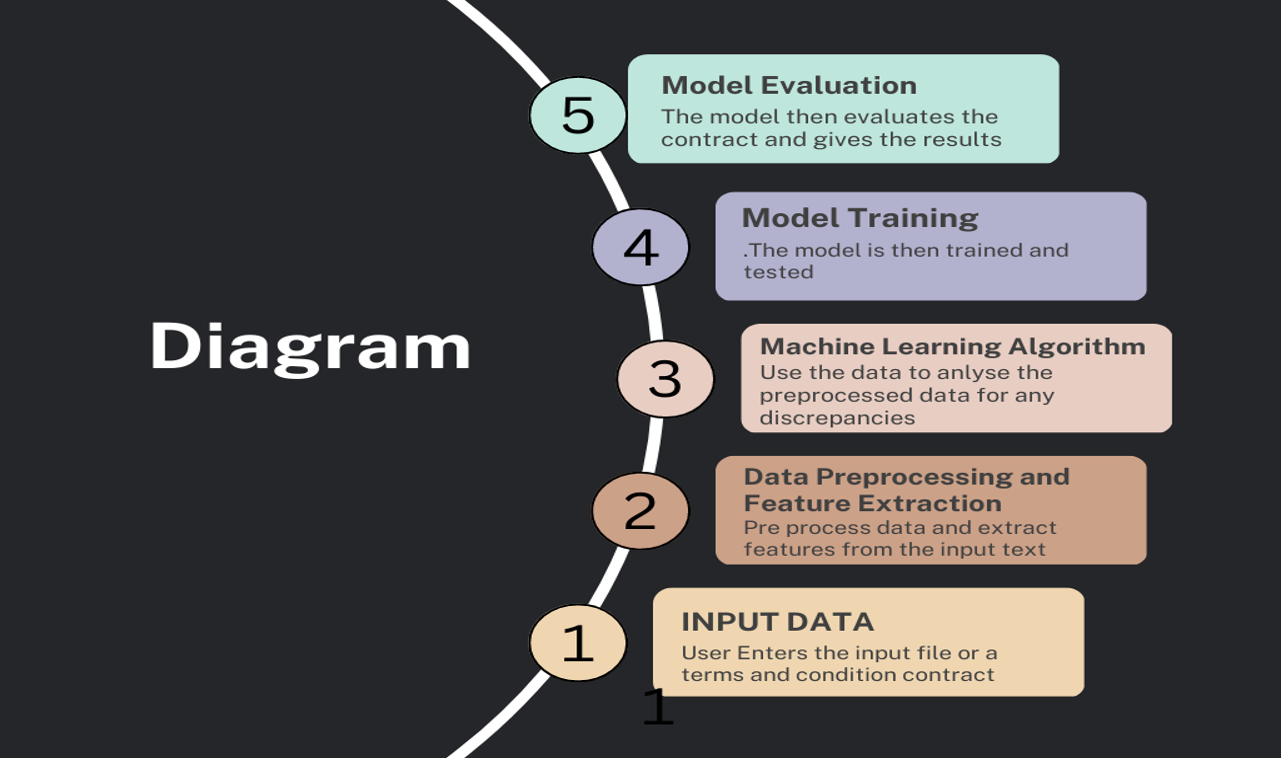
\includegraphics{Figures/Diagramoftheproposedsystem.png}}
\caption{\label{Figure::Diagram Of The Proposed System} Diagram Of The Proposed System  \ref{Figure::Diagram Of The Proposed System}}
\end{figure}





\newpage

\section{Mission Statement \label{Section::Mission Statement} }
The primary purpose of this project is to protect stakeholders from falling victim to deceptive clauses in contracts that may undermine their best interests, either intentionally or unintentionally or via other disruptive means. These clauses could cause harm to the signing party through various means, such as monetary loss or other negative consequences that may impact the livelihood of the concerned stakeholder as a whole. 
The proposed machine learning software system aims to detect and flag such fraudulent clauses in terms and conditions contracts, thus empowering stakeholders to make informed decisions before committing to an agreement. 
By leveraging advanced machine learning algorithms, the system will analyze and identify potential risks in the contract language. This approach ensures that stakeholders are aware of any hidden or obscure terms that could be detrimental to their interests. In addition to enhancing the transparency of contractual agreements upheld in a court of law, the software will enable users to negotiate better terms, minimize potential disputes, and ultimately establish a more secure and trustworthy contractual environment.